\documentclass{amsart}
\usepackage{graphicx}
\graphicspath{{./bn1976/}}
\usepackage{hyperref}
\usepackage{csvsimple}
\usepackage{longtable}
\usepackage{lscape}
\usepackage{epigraph}
\title{End Of The Age of Gaussian Confusion}
\author{Zulfikar Moinuddin Ahmed}
\date{\today}
\begin{document}
\maketitle

\section{Barndorff-Nielsen 1976}

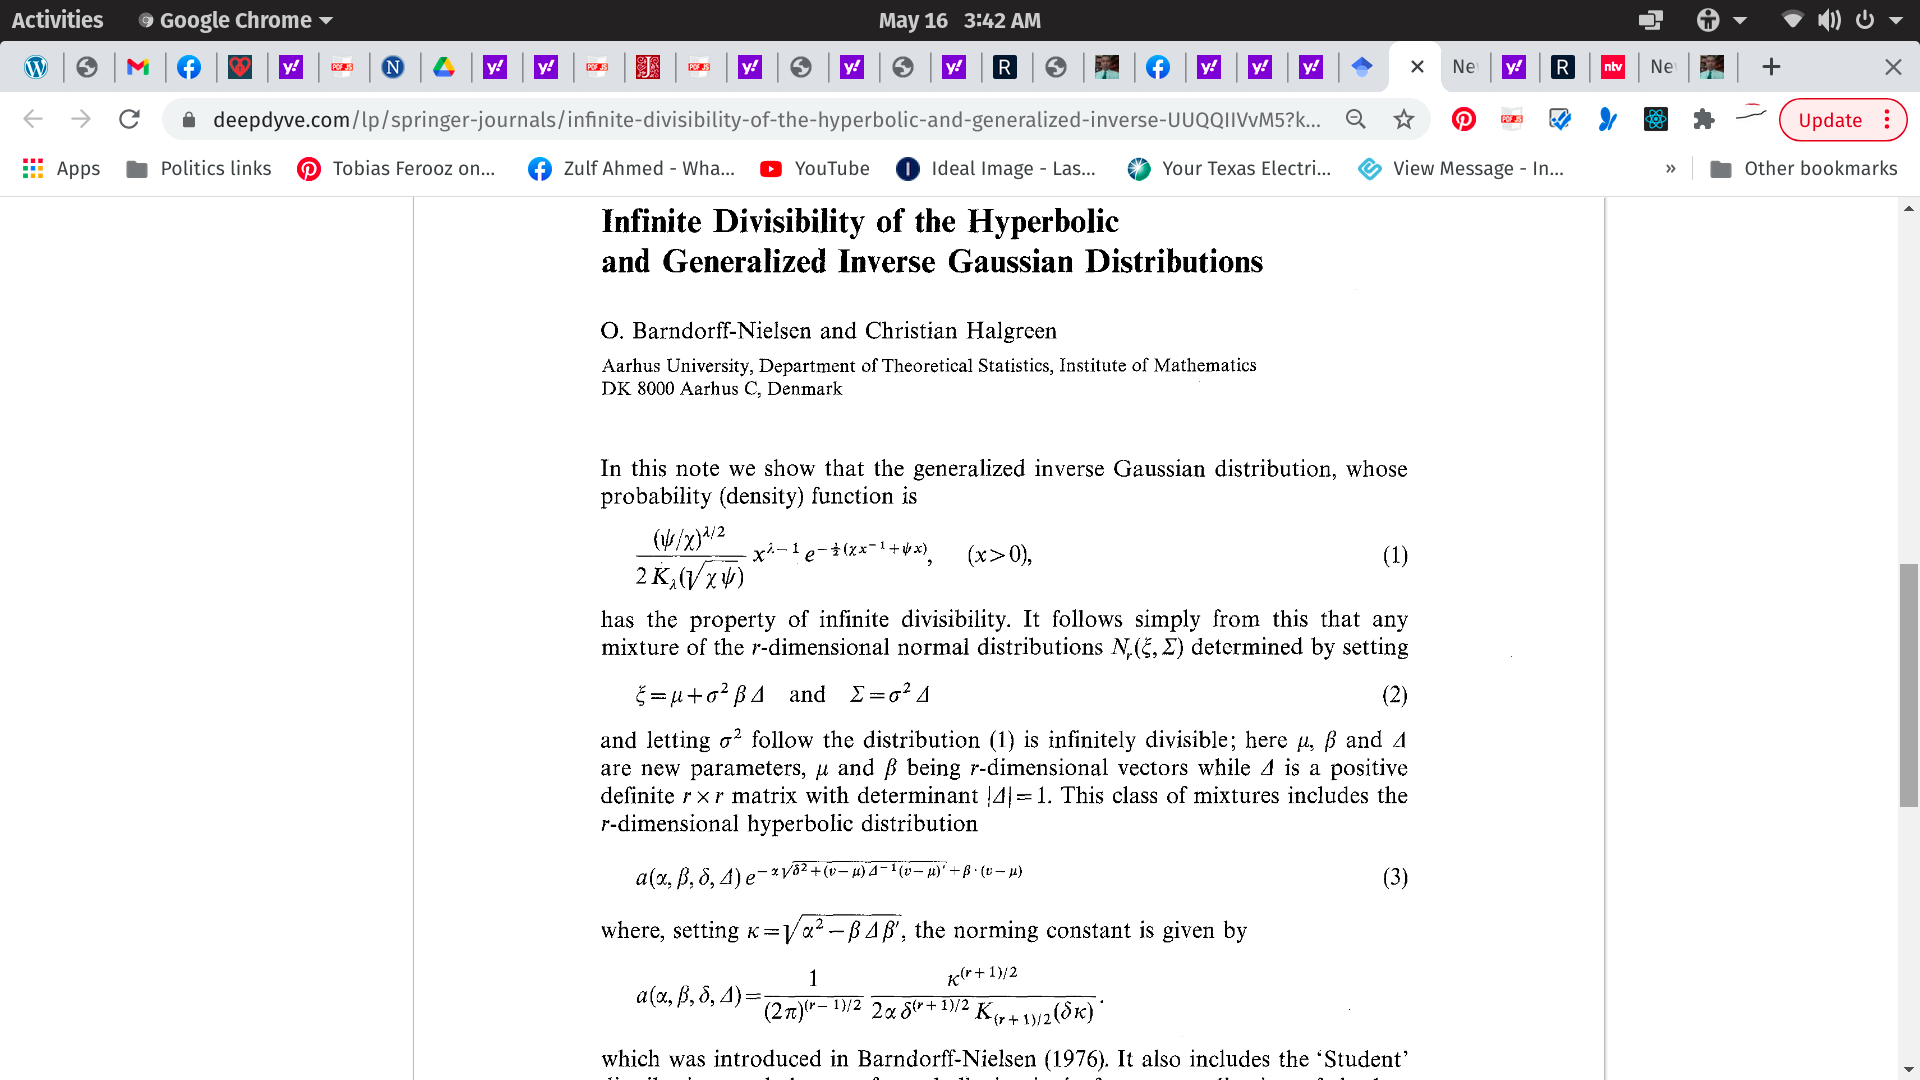
\includegraphics[scale=0.4]{bn1976-1.png}
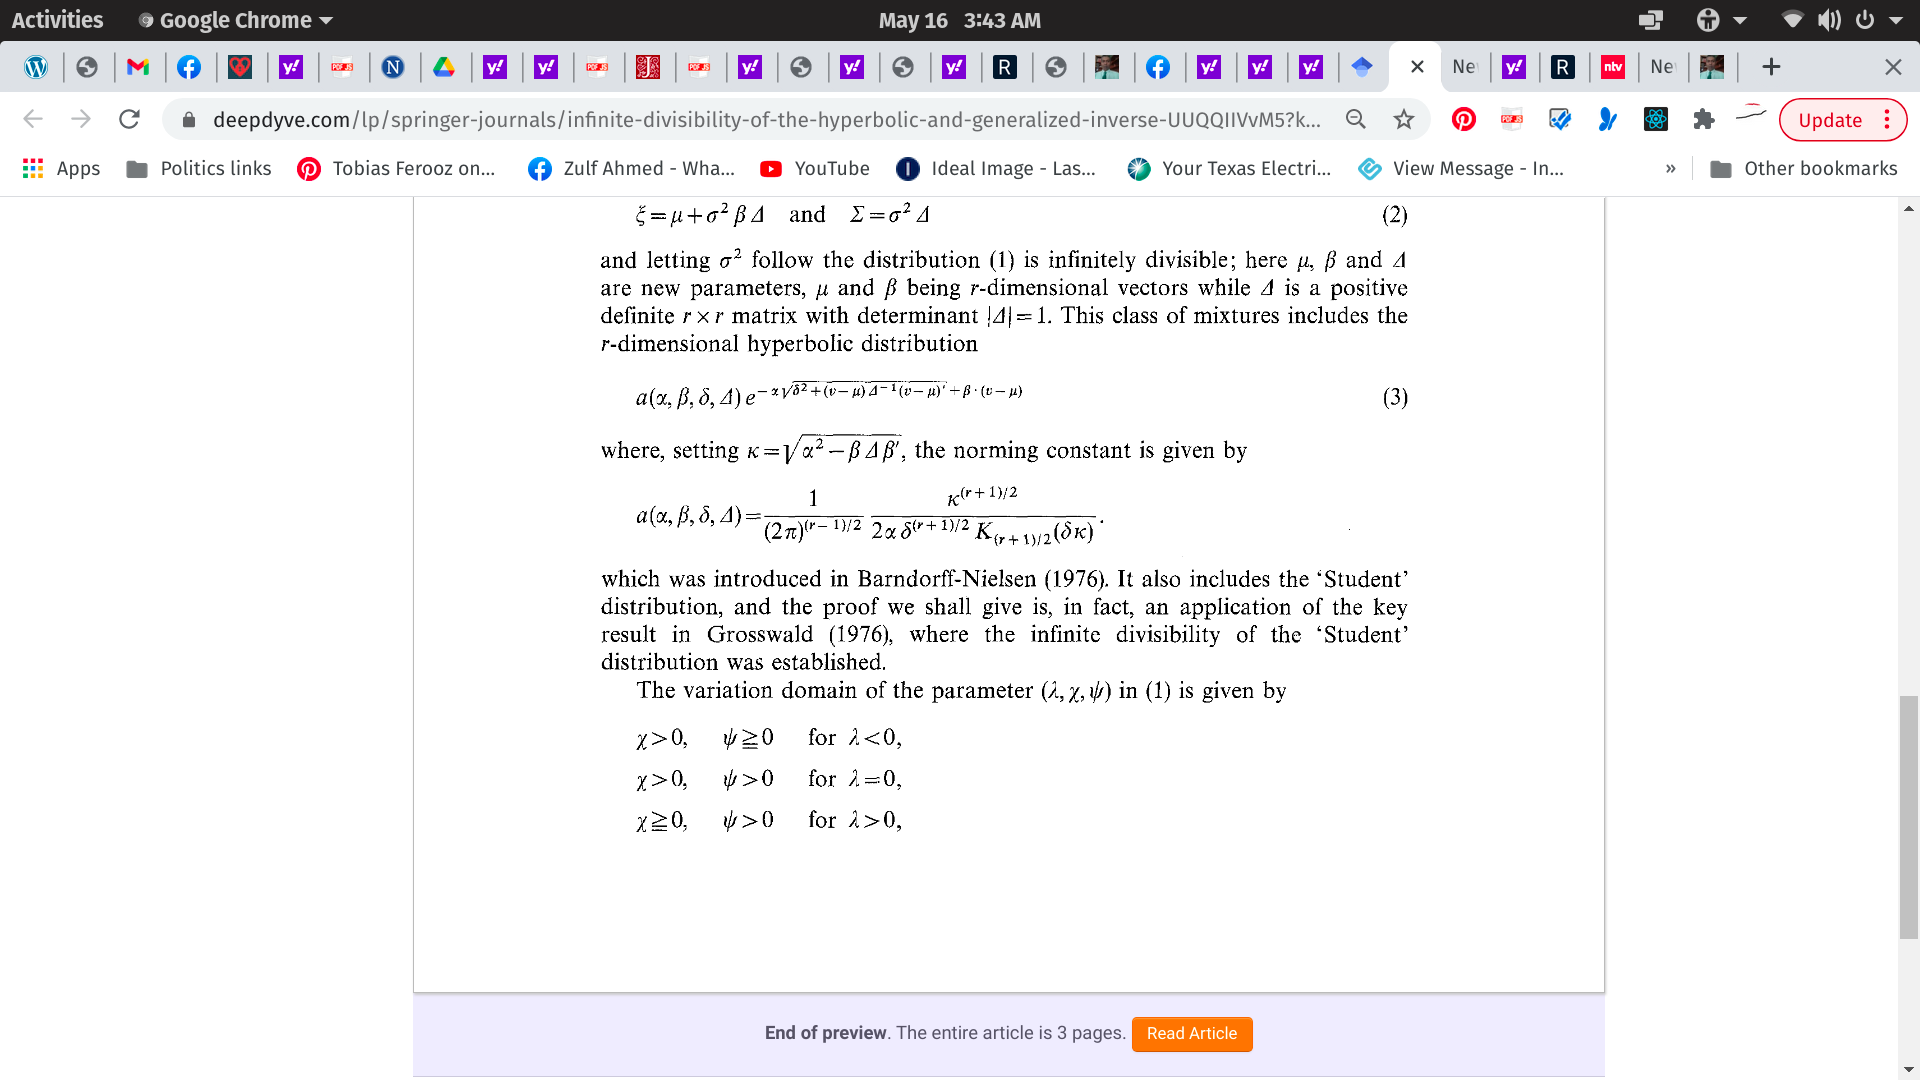
\includegraphics[scale=0.4]{bn1976-2.png}
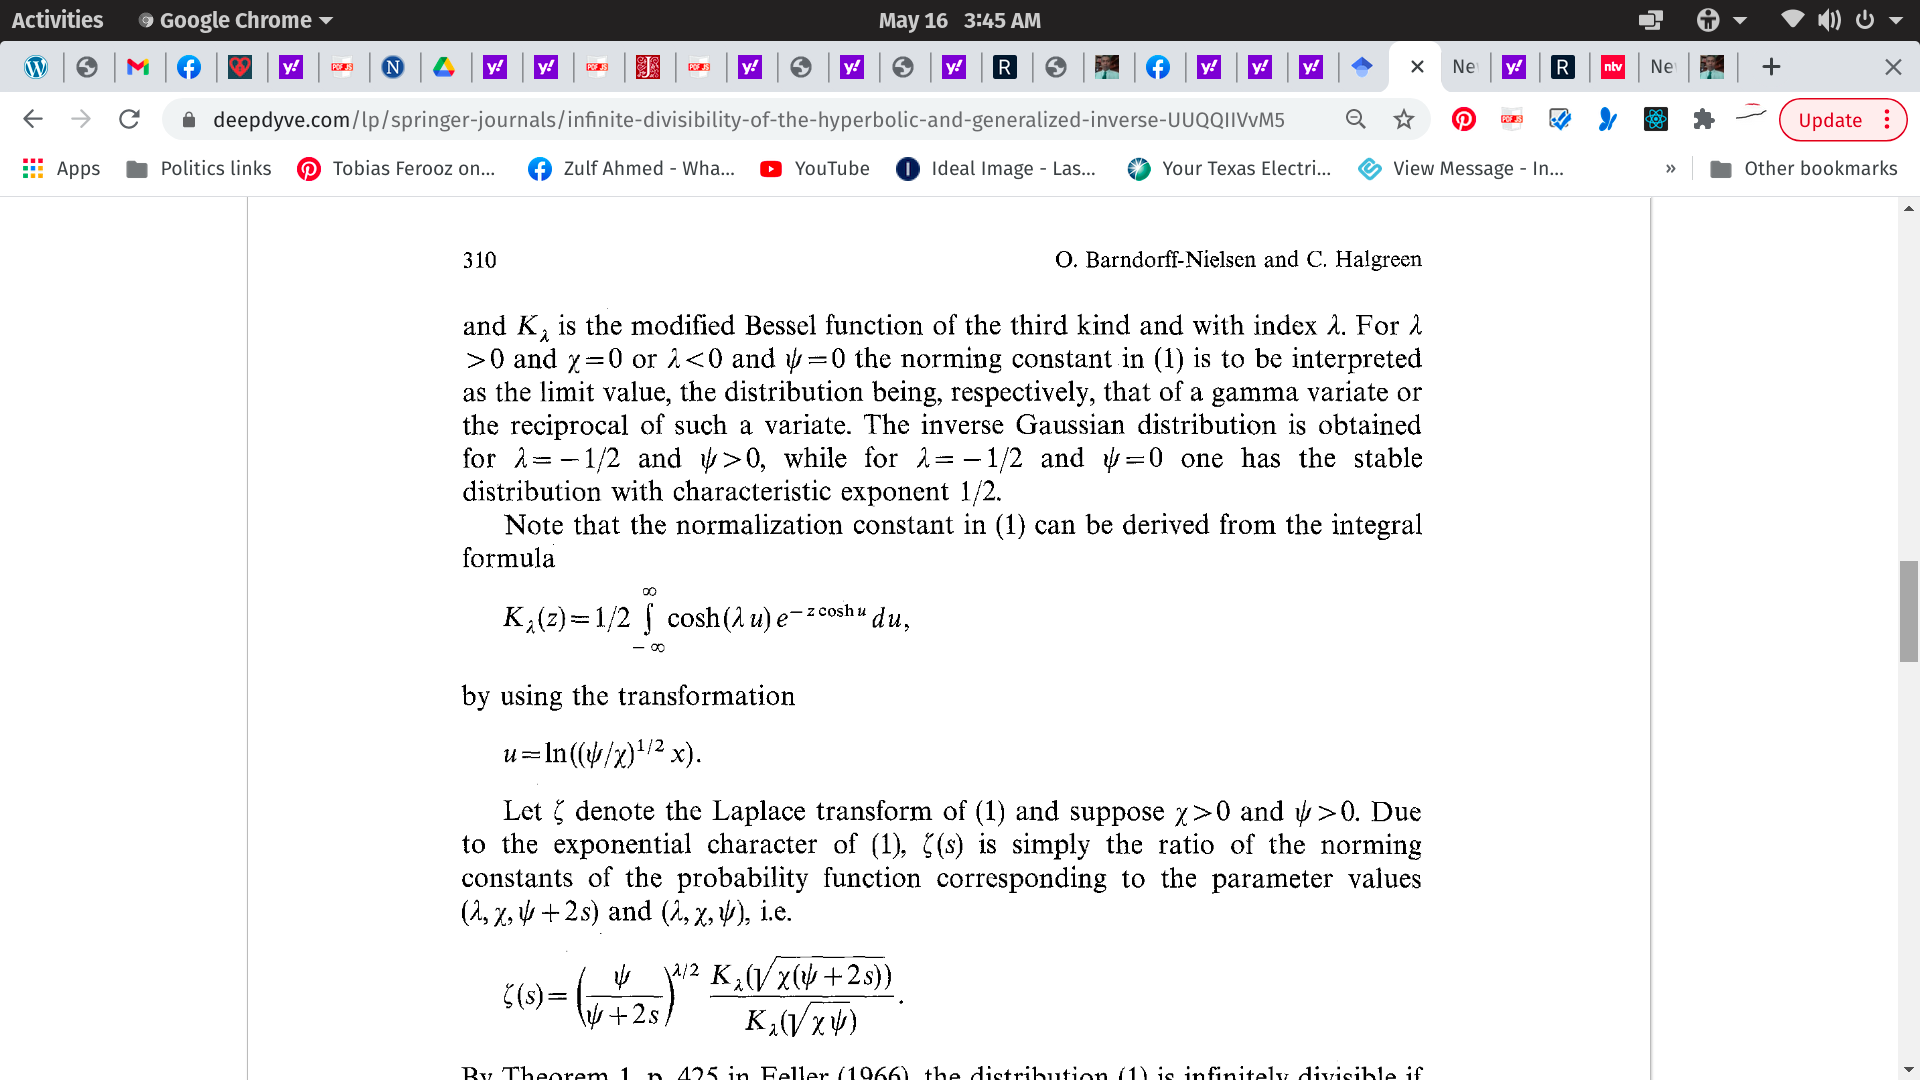
\includegraphics[scale=0.4]{bn1976-3.png}
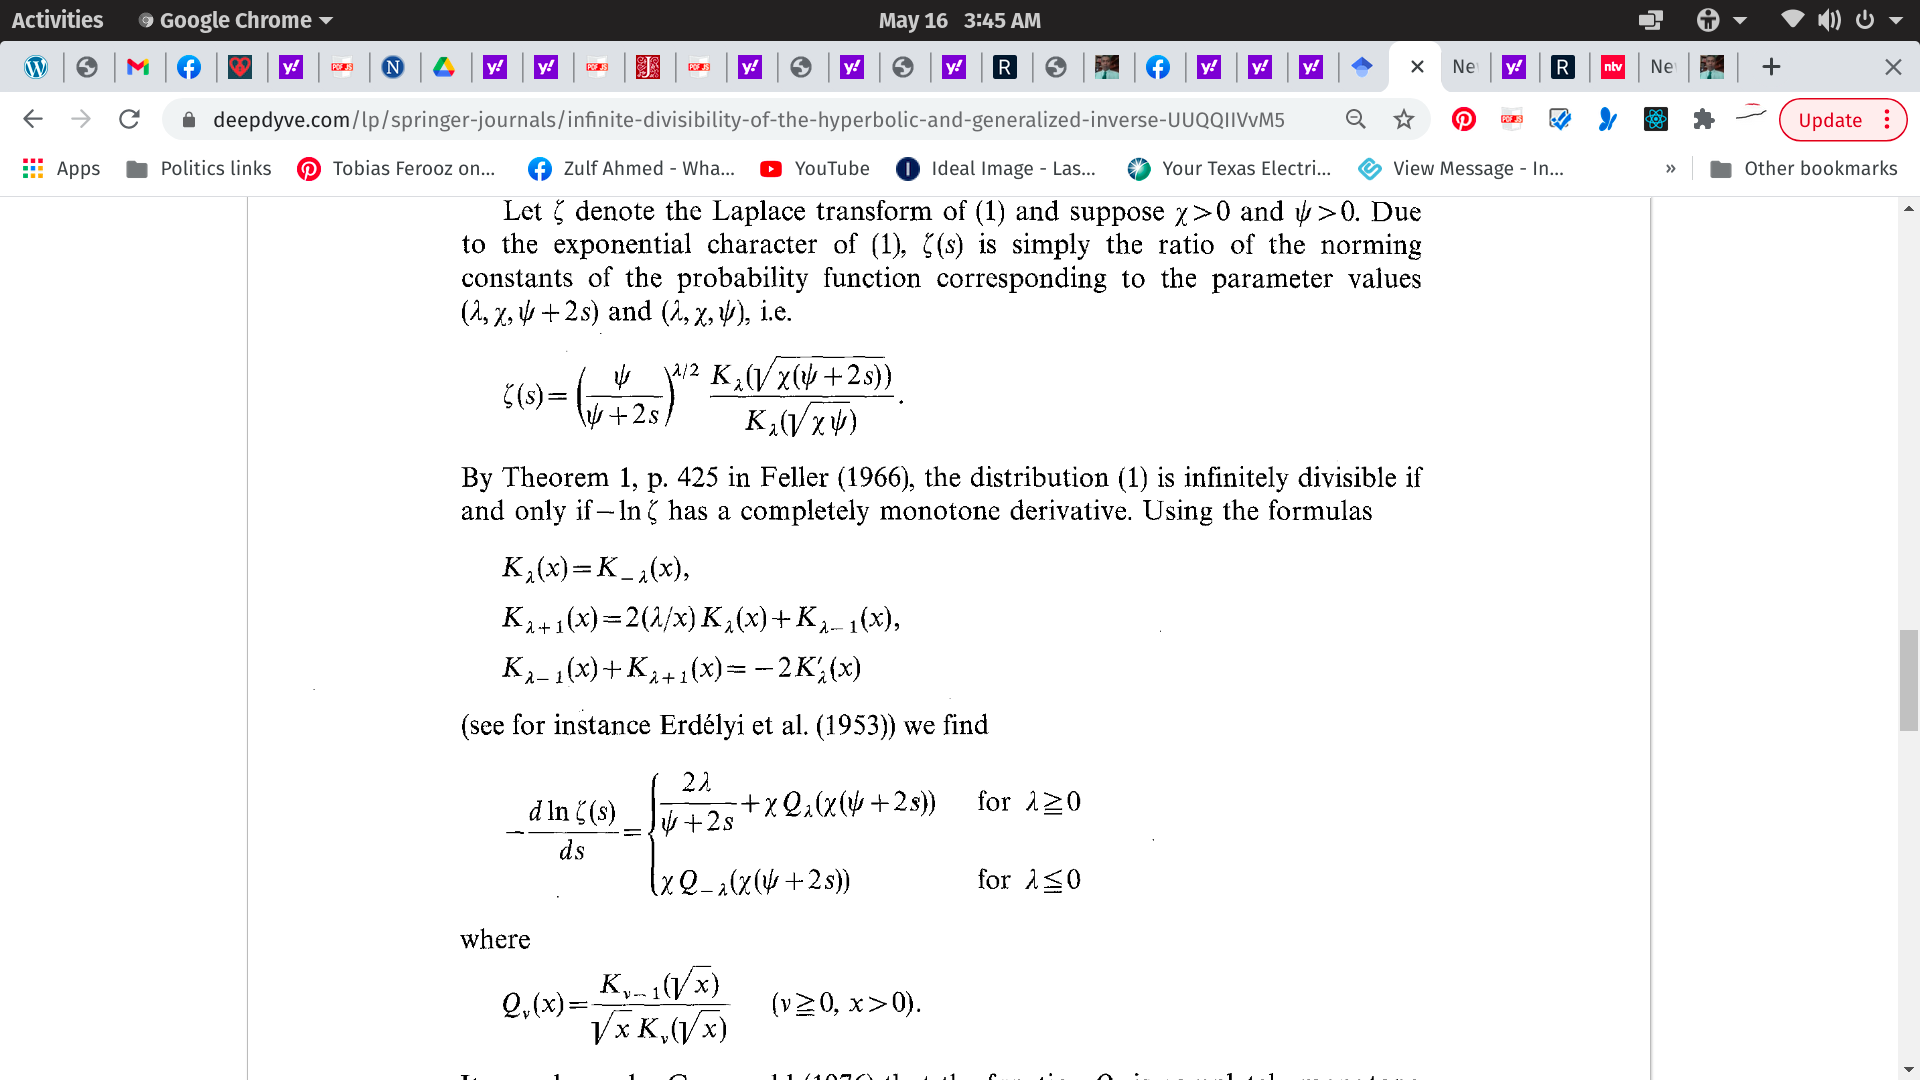
\includegraphics[scale=0.4]{bn1976-4.png}
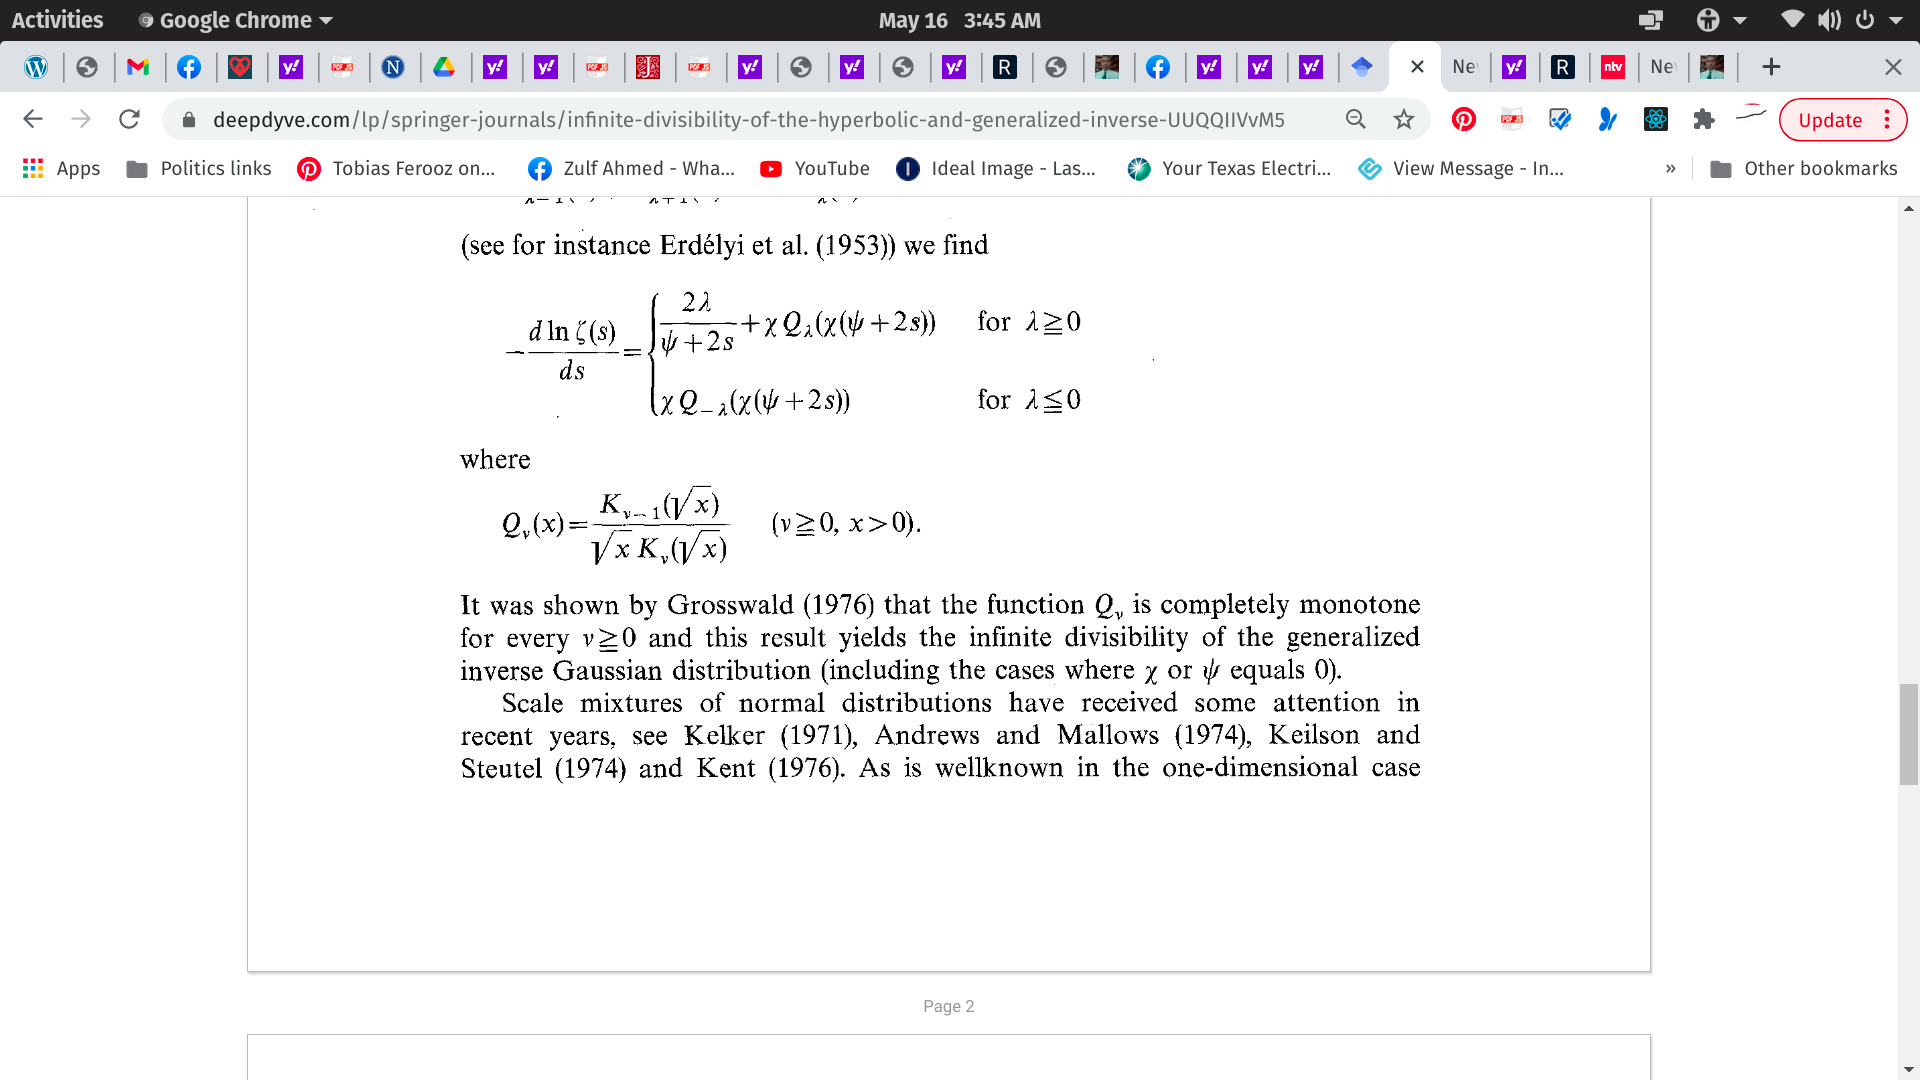
\includegraphics[scale=0.4]{bn1976-5.png}
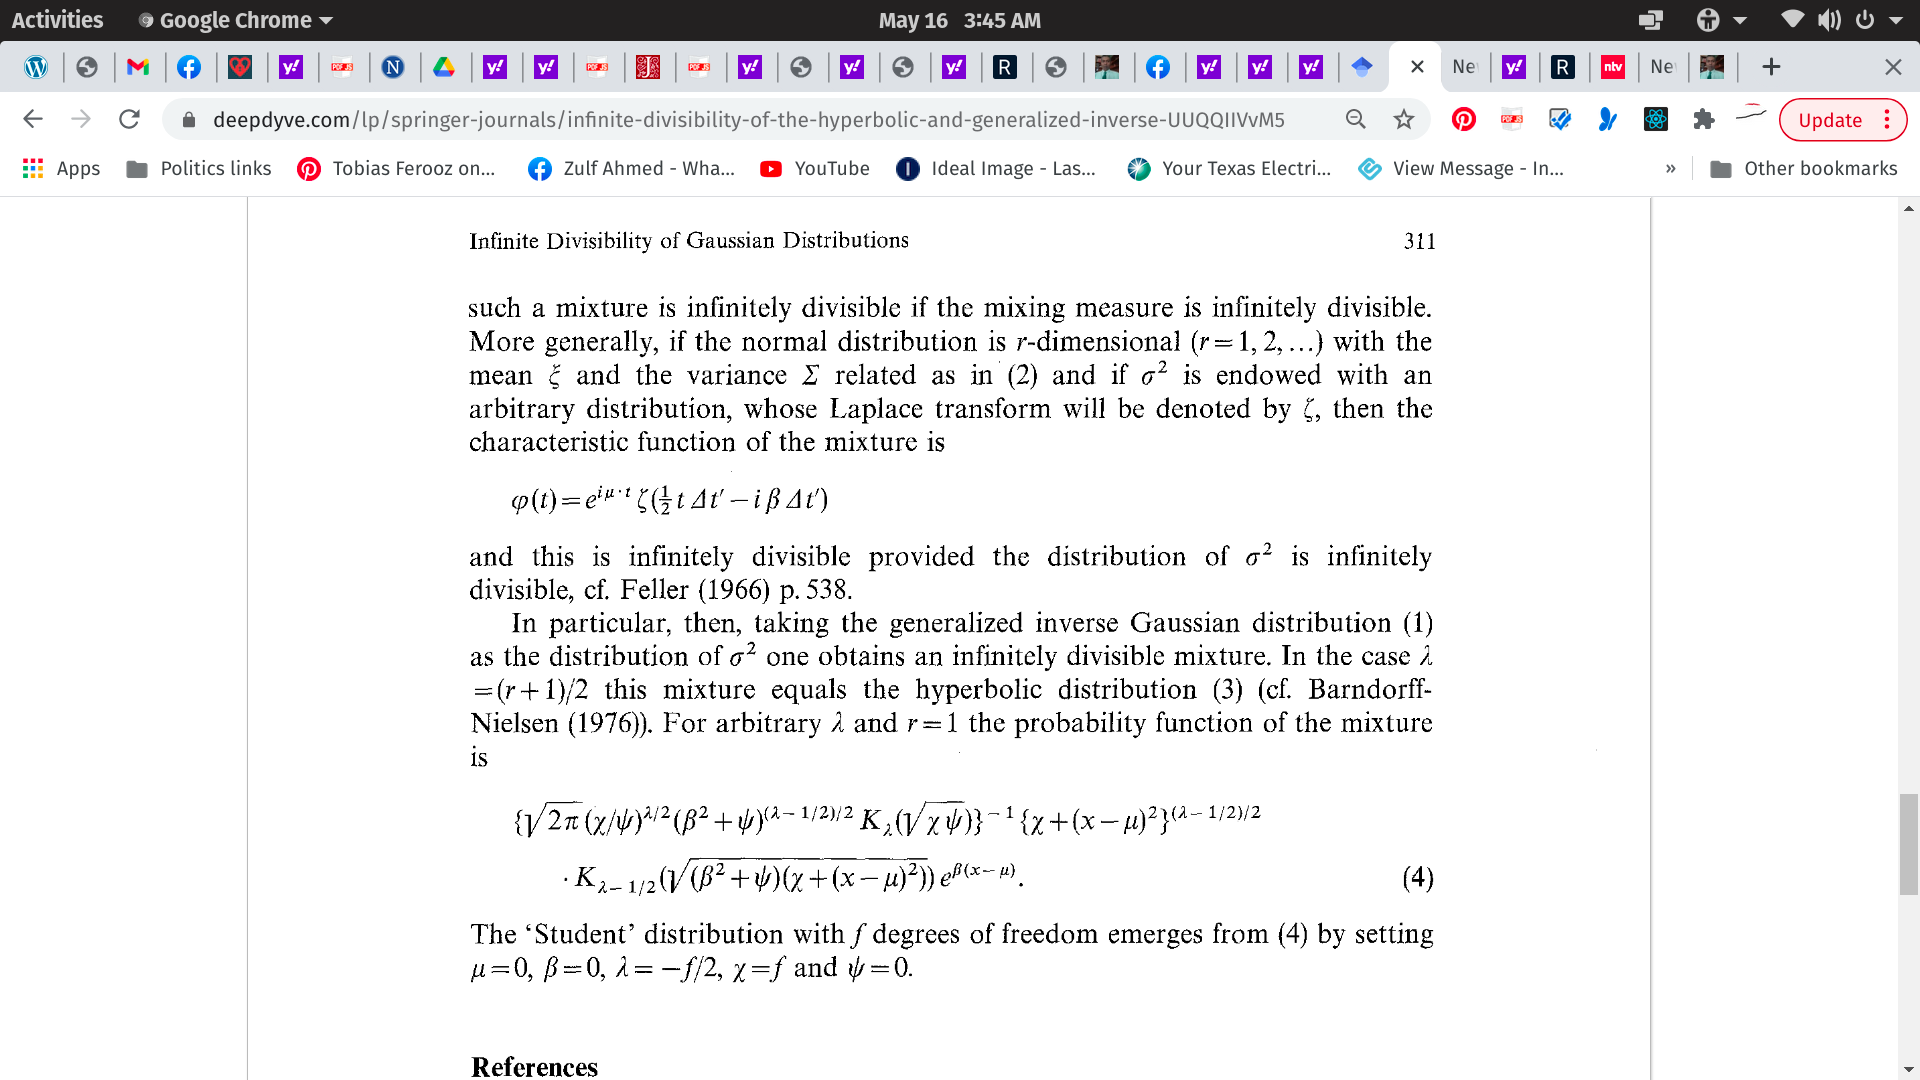
\includegraphics[scale=0.4]{bn1976-6.png}
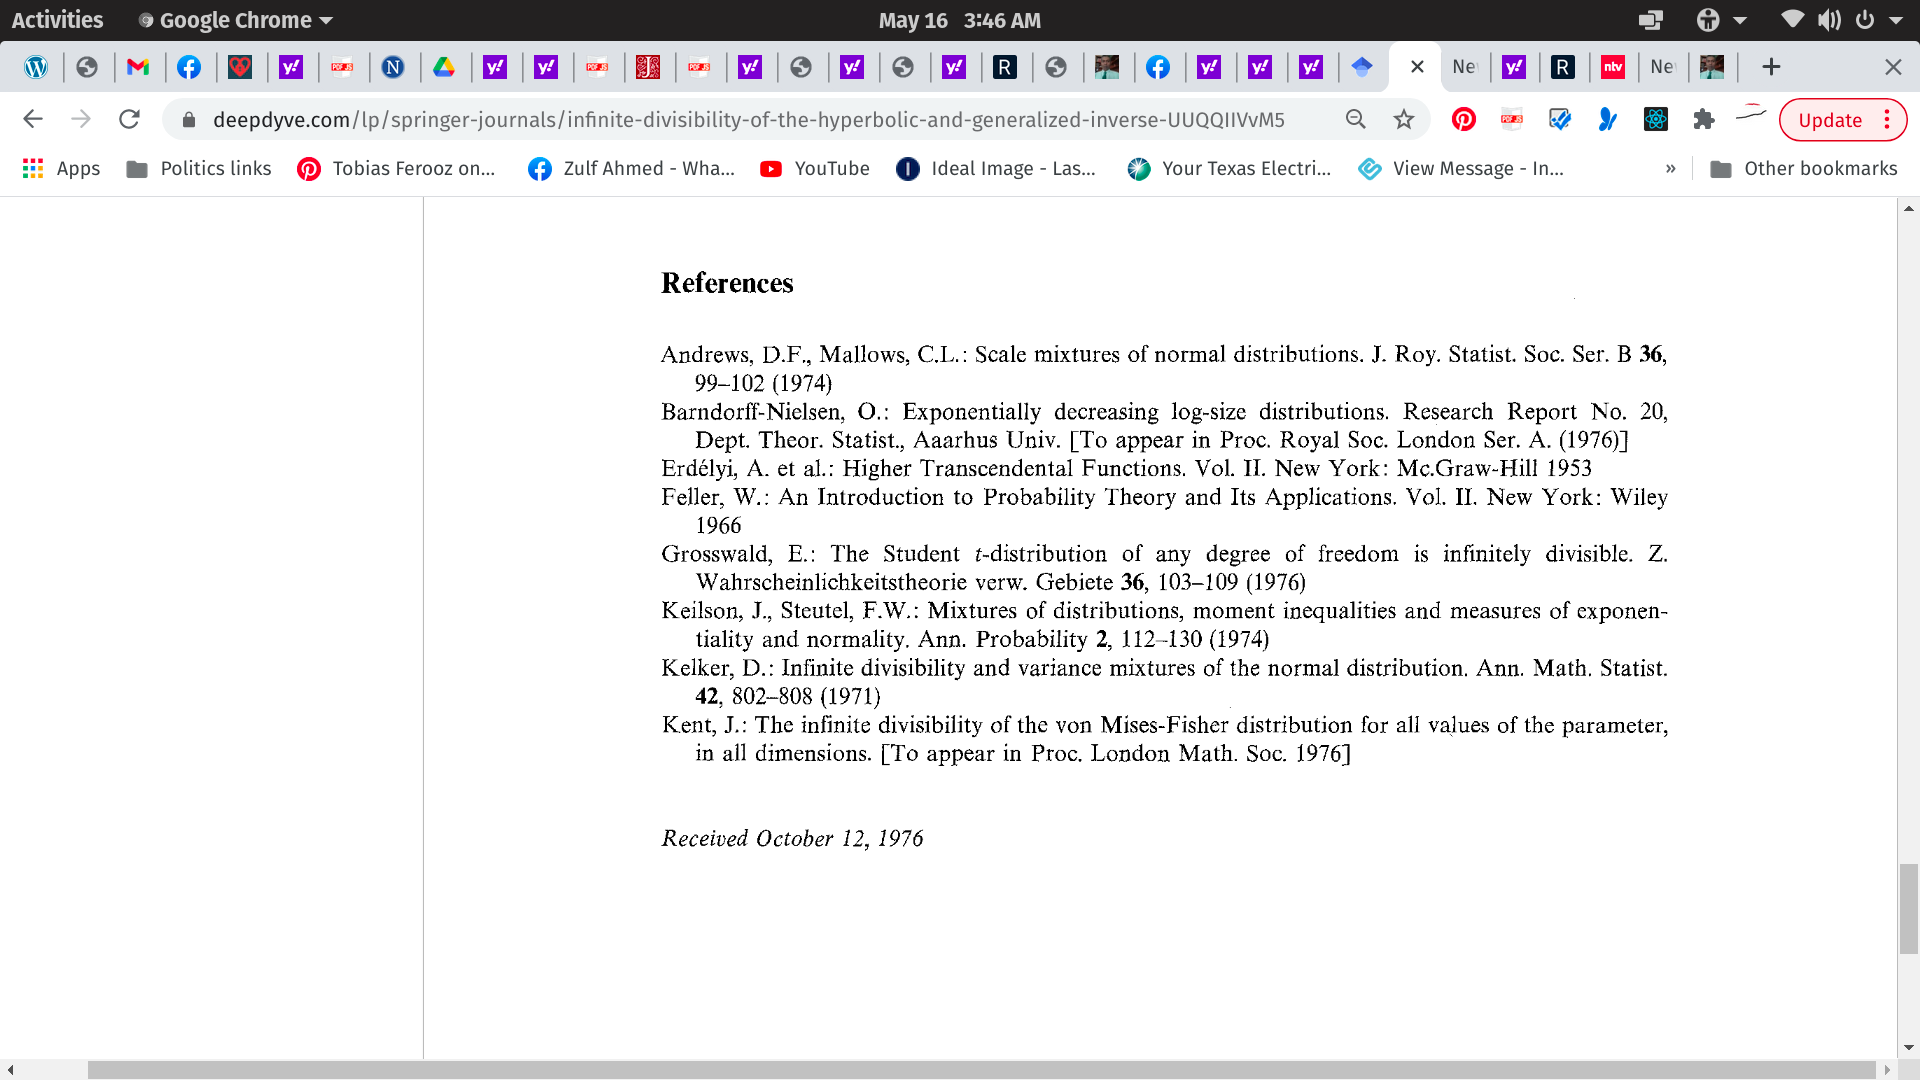
\includegraphics[scale=0.4]{bn1976-7.png}

\section{Two Centuries of Gaussian Confusion In Science}

The pristine beauty of Gaussian distributions and wonderful theory had taken us far.  And it is time to give up our childhood in Science regarding what Noise is in the actual universe rather than in mathematical theory.  And it was in 1976 that Ole Barndorff-Nielsen had proved the {\em infinite divisibility} of one of the deepest secrets of the universe, the Generalised Hyperbolic Distribution, which would one day completely replace all use of Gaussian Distributions in all of Science.  You see Gaussian Distributions were our childhood toys.  They allowed the possibility to produce a coherent mathematical body for Brownian motion.  

But ever since the sixties, if not even before then, there were phenomena that had various non-Gaussian noise.  The terminology developed around Gaussian, and it is dreadful terminology.  "Heavy-tailed" distributions.  As though Nature ought to have followed Gaussian Distribution but did not comply. No this is {\em wrong}.  {\em Gaussian Distribution and Processes are toys}!!  Let there be a new and clearer Age of Science.  Let us celebrate the great discovery of Ole Barndorff-Nielsen and replace all Gaussian Distributions and Processes with these GHD, and obviously I am going to consider the names to be Barndorff-Nielsen Distribution and Nature's fundamental processes to be Barndorff-Nielsen Processes because he is Dane and would not propose it.  Let us celebrate this great transition of an Age of Science.
\end{document}
